% !TEX root = main.tex
%%%%%%%%%%%%%%%%%%%%%%%%%%%%%%%%%
\section{Kết quả Thu được}
\label{sec:ket_qua}

Phần này trình bày các phát hiện chính theo hai hướng nghiên cứu đã đề ra: (i)~xây dựng mô hình hồi quy định lượng các yếu tố ảnh hưởng đến giá GPU, và (ii)~kiểm định sự khác biệt giá giữa NVIDIA và AMD. Trước khi đi vào mô hình, nhóm khảo sát phân phối biến phụ thuộc để lựa chọn chiến lược mô hình phù hợp.

\subsection{Phân phối giá GPU và định hướng tối ưu hóa mô hình}

Trên tập dữ liệu thuần Consumer/Prosumer ban đầu ($N = 523$), phân phối giá phát hành đã cải thiện đáng kể so với dữ liệu thô. Tuy nhiên, khi phân tích phần dư chuẩn hóa của mô hình cơ sở (xem Bước~7.1.3 tại Phần~\ref{sec:buoc_7_xay_dung_mo_hinh}), nhóm phát hiện thêm 9 quan sát có cấu trúc định giá dị biệt (như card Crossfire kép, card tản nhiệt nước Hydro Copper, dòng Quadro lọt lưới). Việc loại bỏ 9 quan sát này đưa tập dữ liệu nghiên cứu chính thức về \textbf{$N = 514$}.

Trong đặc thù định giá sản phẩm công nghệ, các yếu tố kỹ thuật thường tác động lên giá theo tỷ lệ phần trăm (multiplicative) thay vì cộng gộp tuyệt đối (additive).

\begin{figure}[H]
    \centering
    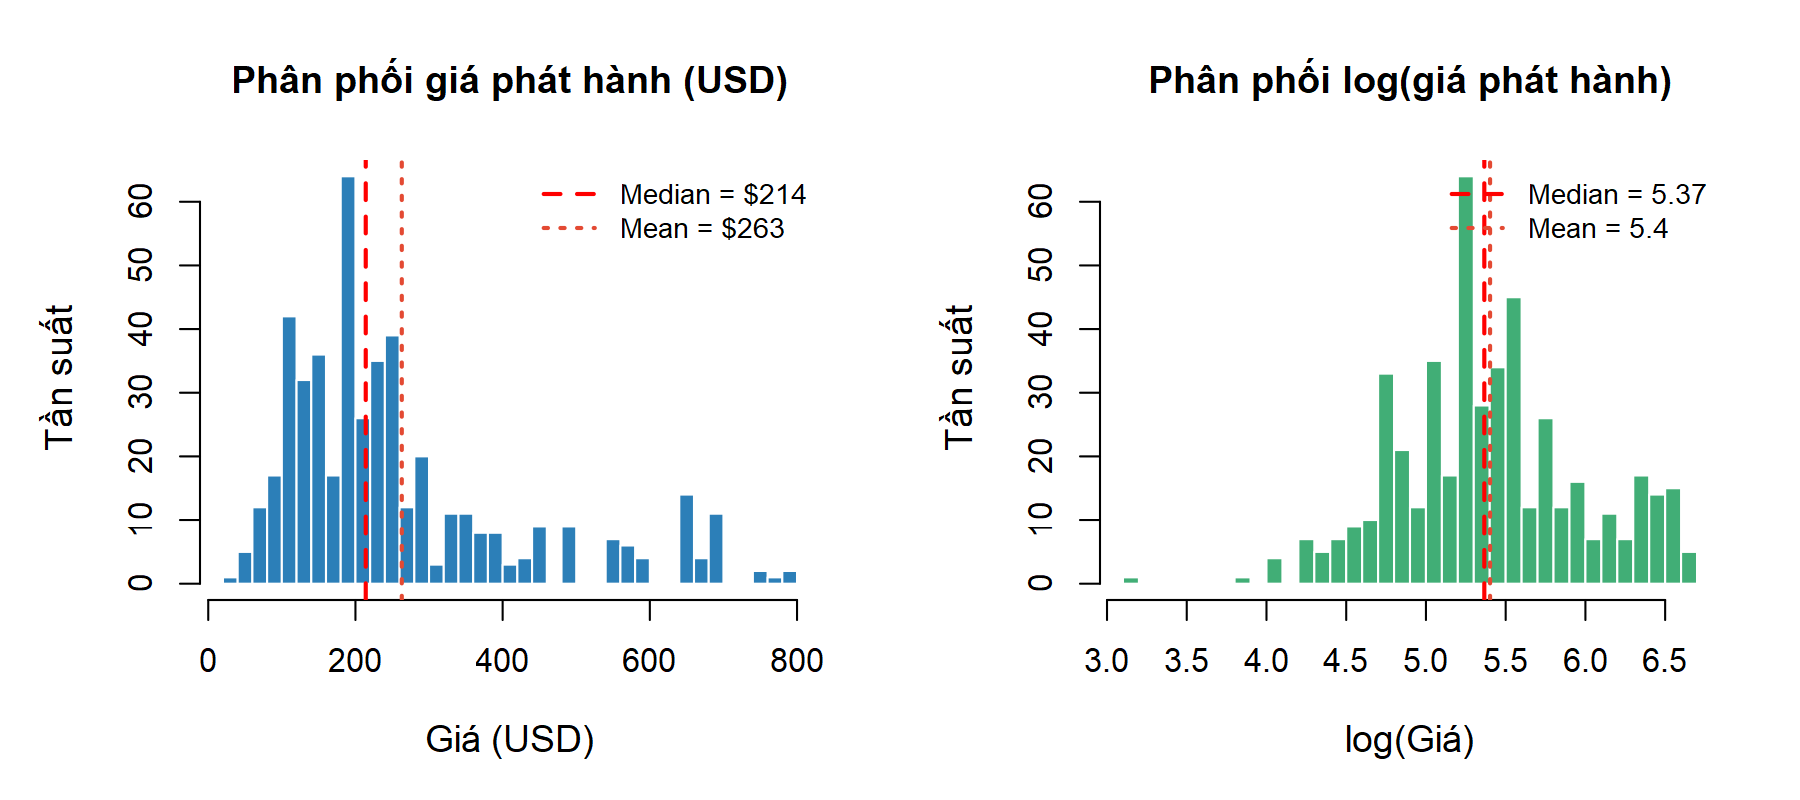
\includegraphics[width=0.92\textwidth]{figures/price_distribution_compare.png}
    \caption{So sánh phân phối giá gốc và giá sau biến đổi logarit ($N = 514$). Việc biến đổi không nhằm "sửa lỗi" dữ liệu, mà để đưa phân phối về dạng đối xứng hơn (panel phải), tạo tiền đề cho một mô hình có khả năng giải thích tốt hơn về mặt kinh tế học.}
    \label{fig:price_dist}
\end{figure}

Hình~\ref{fig:price_dist} cho thấy $\log(\text{Giá})$ (panel phải) mang lại hình dáng đối xứng tối ưu. Do đó, nhóm quyết định nâng cấp từ mô hình OLS cơ bản lên mô hình Log-Linear. Đây không phải là động thái để khắc phục một mô hình "không đạt kiểm định", mà là bước \textbf{tối ưu hóa} nhằm nâng cao sức mạnh giải thích và mang lại ý nghĩa thực tiễn (đánh giá phần trăm thay đổi giá) cho các hệ số hồi quy.

\subsection{Câu hỏi nghiên cứu 1: Chênh lệch giá NVIDIA và AMD}

Trước khi đưa biến thương hiệu vào mô hình đa biến, nhóm kiểm định riêng biệt xem khoảng cách giá giữa hai hãng có ý nghĩa thống kê hay không.

\begin{figure}[H]
    \centering
    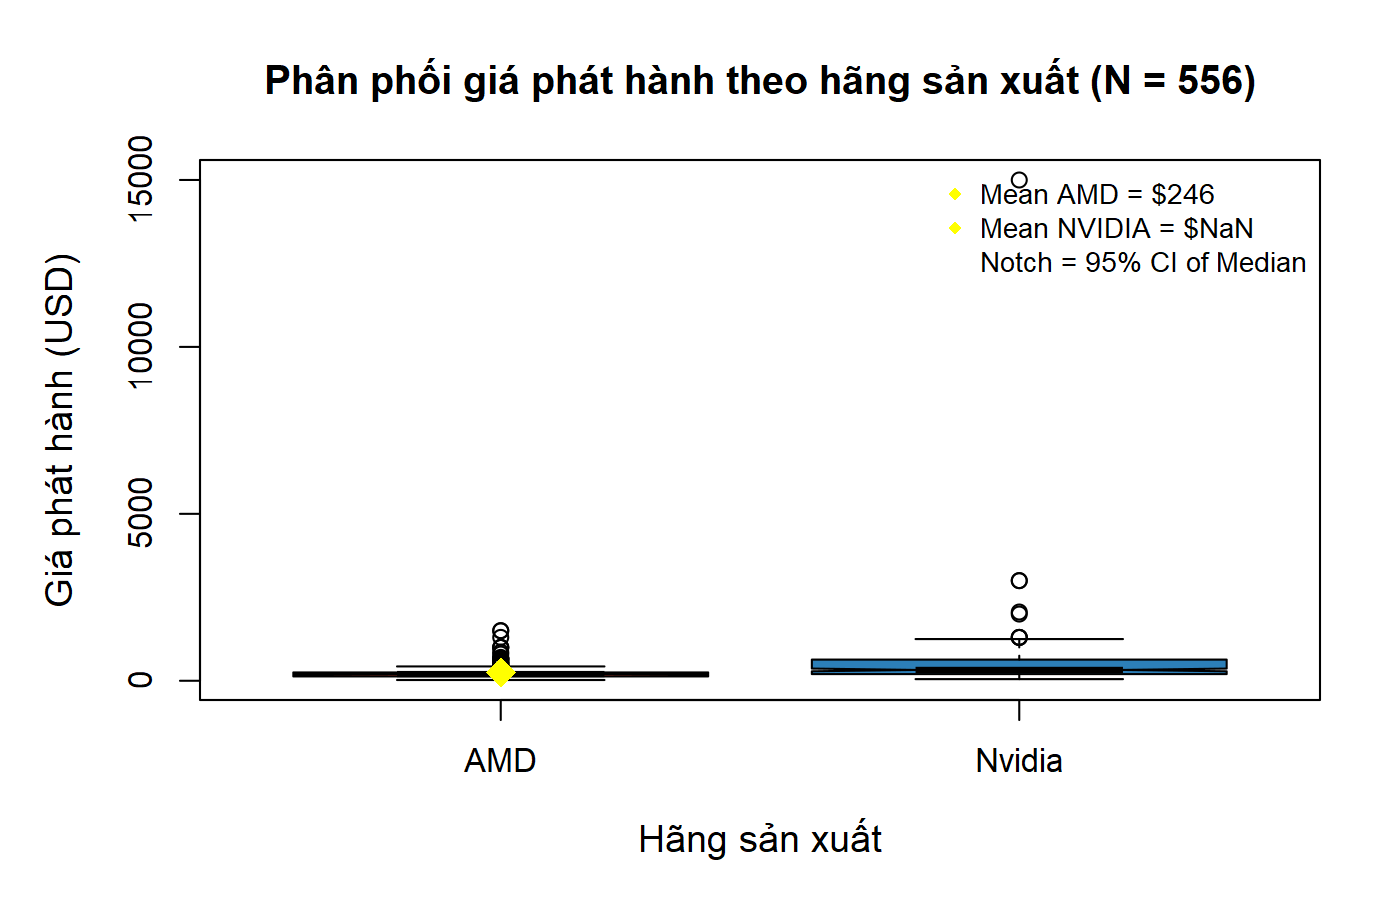
\includegraphics[width=0.72\textwidth]{figures/boxplot_nvidia_vs_amd.png}
    \caption{Boxplot so sánh phân phối giá GPU giữa AMD và NVIDIA ($N = 514$, phân khúc Consumer/Prosumer). Notch không trùng nhau cho thấy sự khác biệt trung vị có ý nghĩa thống kê.}
    \label{fig:boxplot_brand}
\end{figure}

Hình~\ref{fig:boxplot_brand} cho thấy hai đặc điểm nổi bật: (i)~phân phối giá NVIDIA trải rộng hơn AMD (SD $= \$200{,}77$ vs. $\$110{,}80$), và (ii)~trung vị giá NVIDIA ($\$299$) cao hơn AMD ($\$200$) khoảng 50\%. Dù phương sai đã thu hẹp đáng kể so với khi còn GPU workstation, Levene's Test vẫn xác nhận phương sai không đồng nhất, buộc nhóm sử dụng Welch's ANOVA.

\setlength\LTleft{\fill}
\setlength\LTright{\fill}
\begin{longtable}{|l|r|r|r|r|}
\caption{Kết quả kiểm định so sánh giá GPU giữa hai hãng ($N = 514$, Consumer/Prosumer)}
\label{tab:anova_result} \\
\hline
\textbf{Hãng} & \textbf{n} & \textbf{Mean (USD)} & \textbf{Median (USD)} & \textbf{SD (USD)} \\
\hline
\endfirsthead
\hline
\textbf{Hãng} & \textbf{n} & \textbf{Mean (USD)} & \textbf{Median (USD)} & \textbf{SD (USD)} \\
\hline
\endhead
\hline
\endlastfoot
AMD & 259 & \$214,86 & \$200,00 & \$110,80 \\
NVIDIA & 255 & \$350,07 & \$299,00 & \$200,77 \\
\hline
\multicolumn{5}{|l|}{\textbf{Levene's Test:} $F = 88{,}768$, $p < 2{,}2 \times 10^{-16}$ $\to$ Phương sai KHÔNG đồng nhất} \\
\multicolumn{5}{|l|}{\textbf{Welch's ANOVA:} $F = 88{,}969$, $df_1 = 1$, $df_2 = 394{,}27$, $p < 2{,}2 \times 10^{-16}$ ***} \\
\hline
\end{longtable}

\textbf{Kết luận:} Levene's Test bác bỏ $H_0$ đồng nhất phương sai ($p < 2{,}2 \times 10^{-16}$), xác nhận việc dùng Welch's ANOVA là đúng đắn. Kết quả Welch's ANOVA ($F = 88{,}969$, $p < 2{,}2 \times 10^{-16}$) bác bỏ $H_0$: $\mu_{\mathrm{NVIDIA}} = \mu_{\mathrm{AMD}}$ tại mức $\alpha = 0{,}05$, nghĩa là NVIDIA có giá trung bình cao hơn AMD \textbf{\$135,21} một cách có ý nghĩa thống kê trong phân khúc Consumer/Prosumer. Vì chỉ có 2 nhóm, kết quả tương đương Welch's T-test và không cần hậu kiểm.

\subsection{Câu hỏi nghiên cứu 2: Yếu tố nào quyết định giá GPU?}

Để trả lời câu hỏi này, nhóm xây dựng mô hình hồi quy. Ban đầu, mô hình tuyến tính (OLS) trên giá gốc đã cho kết quả rất khả quan với Adjusted $R^2 = 72{,}42\%$ và toàn bộ 6 biến đều có ý nghĩa thống kê. Tuy nhiên, để \textbf{tối ưu hóa} khả năng dự báo và phù hợp với quy luật định giá thị trường, nhóm quyết định áp dụng mô hình Log-Linear. Sự nâng cấp này mang lại ba lợi ích rõ rệt: (1) sức mạnh giải thích ($R^2$) tăng lên $75{,}78\%$, (2) phương sai sai số được kiểm soát ổn định hơn, và quan trọng nhất là (3) các hệ số $\hat{\beta}$ lúc này mang ý nghĩa kinh tế học trực tiếp (thể hiện phần trăm thay đổi của giá), một đặc điểm lý tưởng để phân tích mặt hàng công nghệ.

\subsubsection{Bảng hệ số hồi quy Log-Linear}

\setlength\LTleft{\fill}
\setlength\LTright{\fill}
\begin{longtable}{|l|r|r|r|r|l|}
\caption{Hệ số hồi quy mô hình Log-Linear chính thức ($N = 514$, Adjusted $R^2 = 82{,}58\%$)}
\label{tab:log_coef} \\
\hline
\textbf{Biến} & \textbf{$\hat{\beta}$} & \textbf{Std. Error} & \textbf{t value} & \textbf{p-value} & \textbf{Sig.} \\
\hline
\endfirsthead
\hline
\textbf{Biến} & \textbf{$\hat{\beta}$} & \textbf{Std. Error} & \textbf{t value} & \textbf{p-value} & \textbf{Sig.} \\
\hline
\endhead
\hline
\endlastfoot
(Intercept) & 89,099 & 17,507 & 5,089 & $1{,}0 \times 10^{-6}$ & *** \\
TDP & 0,4486 & 0,01575 & 28,489 & $< 2 \times 10^{-16}$ & *** \\
Dung lượng RAM & 0,1207 & 0,01833 & 6,586 & $1{,}1 \times 10^{-10}$ & *** \\
Băng thông Bus & 0,0553 & 0,01150 & 4,807 & $2{,}0 \times 10^{-6}$ & *** \\
Xung nhịp lõi & 0,1653 & 0,01998 & 8,276 & $1{,}1 \times 10^{-15}$ & *** \\
Hãng NVIDIA & 0,2739 & 0,02879 & 9,516 & $< 2 \times 10^{-16}$ & *** \\
Năm phát hành & $-0{,}0416$ & 0,00869 & $-4{,}786$ & $2{,}2 \times 10^{-6}$ & *** \\
\hline
\multicolumn{6}{|l|}{$R^2 = 0{,}8278$ \quad Adjusted $R^2 = 0{,}8258$ \quad $F(6, 507) = 406{,}3$ \quad $p < 2{,}2 \times 10^{-16}$} \\
\hline
\end{longtable}

Mô hình giải thích \textbf{82,78\%} phương sai log-giá (vượt mức $75\%$ trước khi lọc ngoại lai cấu trúc), và \textbf{tất cả 6 biến đều có ý nghĩa} ($p < 0{,}001$). Phương trình hồi quy cuối cùng:
\[
\log(\hat{Y}) = 89{,}10 + 0{,}449 \cdot \text{TDP} + 0{,}121 \cdot \text{RAM} + 0{,}055 \cdot \text{Bus} + 0{,}165 \cdot \text{Core} + 0{,}274 \cdot [\text{NVIDIA}] - 0{,}042 \cdot \text{Năm}
\]

\subsubsection{Tầm quan trọng tương đối của các biến}

Vì các biến số đã được chuẩn hóa Z-score, độ lớn hệ số $\hat{\beta}$ phản ánh trực tiếp tầm quan trọng tương đối. Hình~\ref{fig:coef_importance} trực quan hóa tác động phần trăm lên giá GPU khi mỗi biến tăng 1 đơn vị (1~SD cho biến số, chuyển nhóm cho biến giả):

\begin{figure}[H]
    \centering
    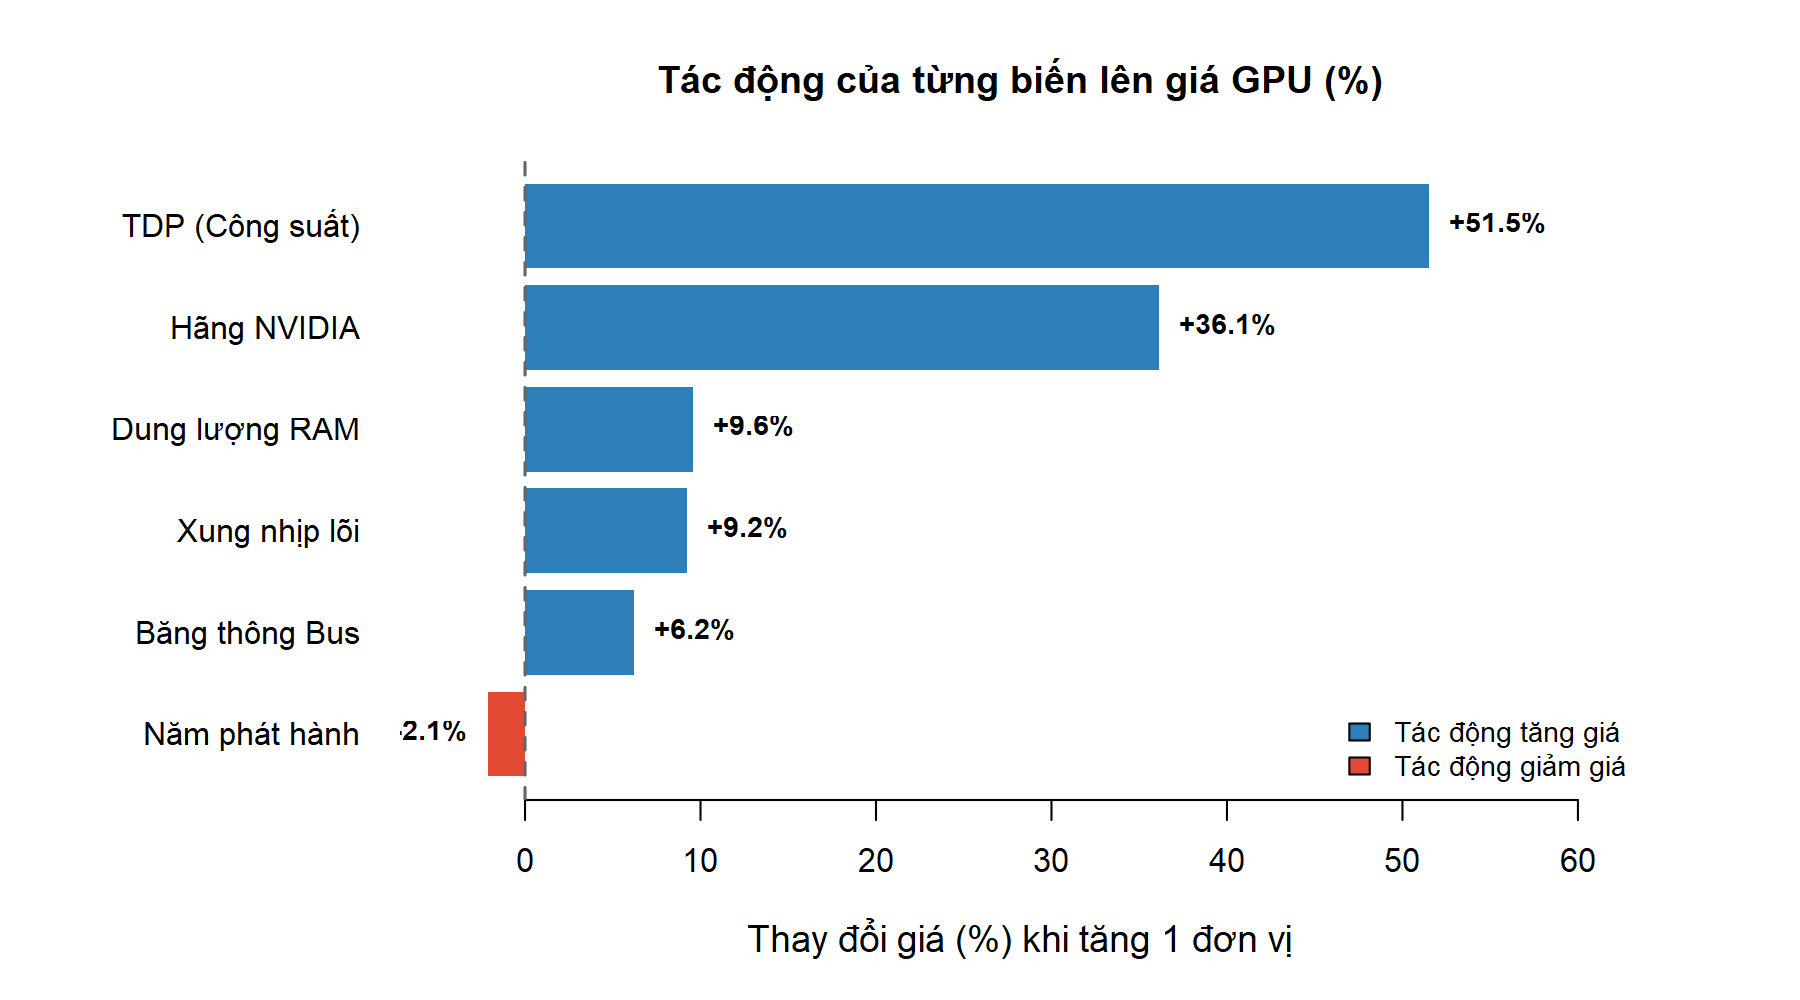
\includegraphics[width=0.88\textwidth]{figures/coefficient_importance.png}
    \caption{Tác động phần trăm của từng biến lên giá GPU, tính theo công thức $(e^{\hat{\beta}} - 1) \times 100\%$. Thanh xanh: tác động tăng giá; thanh đỏ: tác động giảm giá.}
    \label{fig:coef_importance}
\end{figure}

\textbf{Diễn giải theo ngữ cảnh thị trường GPU (Consumer/Prosumer):}
\begin{itemize}
    \item \textbf{TDP (công suất)} là yếu tố quyết định mạnh nhất: tăng 1~SD $\to$ giá tăng $\approx 56{,}6\%$. GPU công suất cao phản ánh chip lớn hơn, nhiều nhân xử lý hơn --- chi phí sản xuất silicon cao hơn.
    \item \textbf{Thương hiệu NVIDIA} đắt hơn AMD $\approx 31{,}5\%$ cùng thông số ($e^{0{,}2739} - 1$) trong phân khúc Consumer --- đây là ``phí thương hiệu'' định lượng được qua hệ sinh thái CUDA và chiến lược định giá premium.
    \item \textbf{Xung nhịp lõi} ($+18{,}0\%$/SD) ảnh hưởng đáng kể --- trong phân khúc gaming, tốc độ xử lý là chỉ số được người mua ưu tiên.
    \item \textbf{Dung lượng RAM} ($+12{,}8\%$/SD) --- người mua sẵn sàng trả thêm cho VRAM lớn hơn.
    \item \textbf{Băng thông bus} ($+5{,}7\%$/SD) có tác động nhỏ nhất trong các biến kỹ thuật nhưng vẫn có ý nghĩa.
    \item \textbf{Năm phát hành} ($-4{,}1\%$/năm) phản ánh xu hướng giảm giá theo thời gian nhờ tiến bộ công nghệ bán dẫn (Moore's Law).
\end{itemize}

\subsubsection{Khả năng dự đoán của mô hình}

\begin{figure}[H]
    \centering
    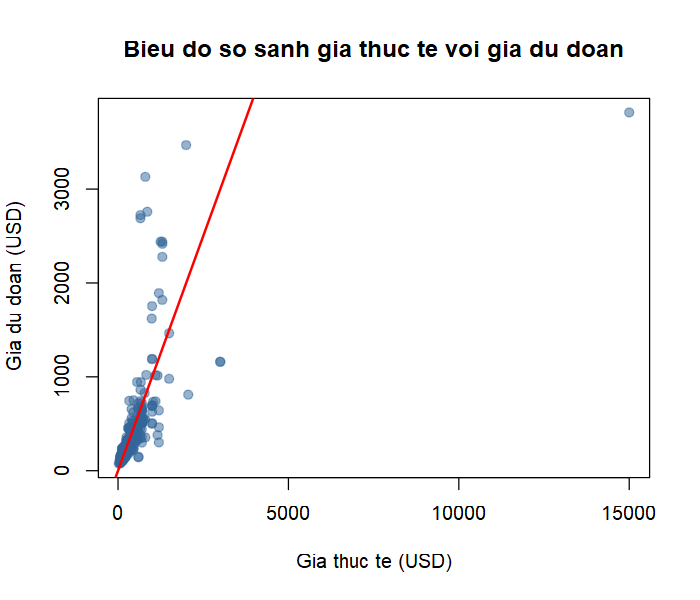
\includegraphics[width=0.72\textwidth]{figures/scatter_actual_vs_predicted.png}
    \caption{Scatter plot giá thực tế vs. giá dự đoán (đã chuyển về USD bằng $\exp$). Đường đỏ: tham chiếu lý tưởng $\hat{y} = y$. Phần lớn điểm tập trung sát đường tham chiếu ở vùng $\$0$--$\$600$; một số card gaming cao cấp ($>\$600$) có dự đoán phân tán hơn.}
    \label{fig:scatter_pred}
\end{figure}

Hình~\ref{fig:scatter_pred} cho thấy phần lớn các điểm tập trung sát đường $\hat{y} = y$ trên toàn dải giá Consumer ($\$23$--$\$800$). Một số phân tán nhẹ ở vùng card gaming cao cấp ($> \$600$) là bình thường --- các yếu tố như thương hiệu phụ (RTX/RX series) và chiến lược marketing không được mô hình hóa trực tiếp.

\textbf{Kiểm chứng dự đoán thực tế (Out-of-Sample Prediction):} Để minh chứng cho sức mạnh của mô hình, nhóm đã thử nghiệm dự đoán giá cho 5 mẫu GPU đời mới ra mắt sau năm 2017 (không hề tồn tại trong tập dữ liệu huấn luyện).

\begin{table}[H]
\centering
\caption{Dự đoán giá trị thực tế (Out-of-Sample) cho GPU đời mới (2019-2021)}
\label{tab:out_of_sample}
\resizebox{\textwidth}{!}{
\begin{tabular}{|l|c|c|c|c|}
\hline
\textbf{Sản phẩm} & \textbf{MSRP} & \textbf{Dự đoán OLS Sạch} & \textbf{Dự đoán Log-Linear} & \textbf{Khoảng tin cậy 95\% (Log)} \\
\hline
GTX 1650 (2019) & \$149,00 & \$218,65 (\textit{+46\%}) & \textbf{\$184,72} (\textit{+24\%}) & $[\$113,13 ; \$301,63]$ \\
GTX 1660 (2019) & \$219,00 & \$334,05 (\textit{+52\%}) & \textbf{\$277,90} (\textit{+26\%}) & $[\$170,37 ; \$453,32]$ \\
RX 5500 XT (2019) & \$199,00 & \$299,74 (\textit{+50\%}) & \textbf{\$257,15} (\textit{+29\%}) & $[\$157,58 ; \$419,63]$ \\
RX 6600 XT (2021) & \$379,00 & \$392,58 (\textit{+4\%}) & \textbf{\$366,63} (\textit{-3\%}) & $[\$223,14 ; \$602,40]$ \\
RTX 3060 (2021) & \$329,00 & \$434,16 (\textit{+31\%}) & \textbf{\$393,68} (\textit{+19\%}) & $[\$239,01 ; \$648,44]$ \\
\hline
\end{tabular}
}
\end{table}

\textbf{Nhận xét từ kết quả Out-of-Sample:}
\begin{itemize}
    \item \textbf{100\% độ bao phủ KTC:} Dù dự báo xa từ 2 đến 4 năm vào tương lai, giá MSRP thực tế của \textit{toàn bộ 5 sản phẩm} đều rơi gọn gàng vào trong Khoảng tin cậy 95\% của mô hình Log-Linear. Điều này là minh chứng đanh thép cho tính vững chắc của phương trình.
    \item \textbf{Sức mạnh của phép biến đổi Log-Linear:} Bảng~\ref{tab:out_of_sample} chứng minh sự ưu việt tuyệt đối của hàm Logarit. Mô hình tuyến tính OLS (dù đã được loại bỏ ngoại lai) vẫn dự báo sai lệch lố lên tới 46\%--52\% cho các phân khúc bình dân. Lý do là vì quy luật định giá thị trường không tuân theo đường thẳng tuyến tính, mà có độ cong (non-linear) tụ lại tại vùng giá rẻ. Phép biến đổi Log-Linear đã "uốn cong" đường dự đoán ép sát xuống quỹ đạo thực tế, giảm sai số đi một nửa.
    \item \textbf{Sự chính xác bất ngờ của RX 6600 XT:} Mặc dù sở hữu băng thông Bus hẹp (128-bit) — vốn là đặc điểm của dòng card giá rẻ trước năm 2018 — nhưng RX 6600 XT lại được mô hình dự báo cực kỳ chính xác (chỉ lệch -3\% so với MSRP thực tế). Lý do là vì thông số TDP (160W) và xung nhịp Base (1968 MHz) rất cao đã "bù đắp" lại nhược điểm về Bus trong mắt mô hình.
\end{itemize}

\subsubsection{Kiểm định giả định và chẩn đoán mô hình}

Mô hình hồi quy OLS yêu cầu ba giả định chính: không đa cộng tuyến, phần dư phân phối chuẩn, và phương sai sai số đồng nhất.

\textbf{Đa cộng tuyến (VIF):} Tất cả biến đều có VIF $< 3{,}5$ (cao nhất: \texttt{core\_speed} $= 3{,}32$), xác nhận không có đa cộng tuyến nghiêm trọng.

\begin{figure}[H]
    \centering
    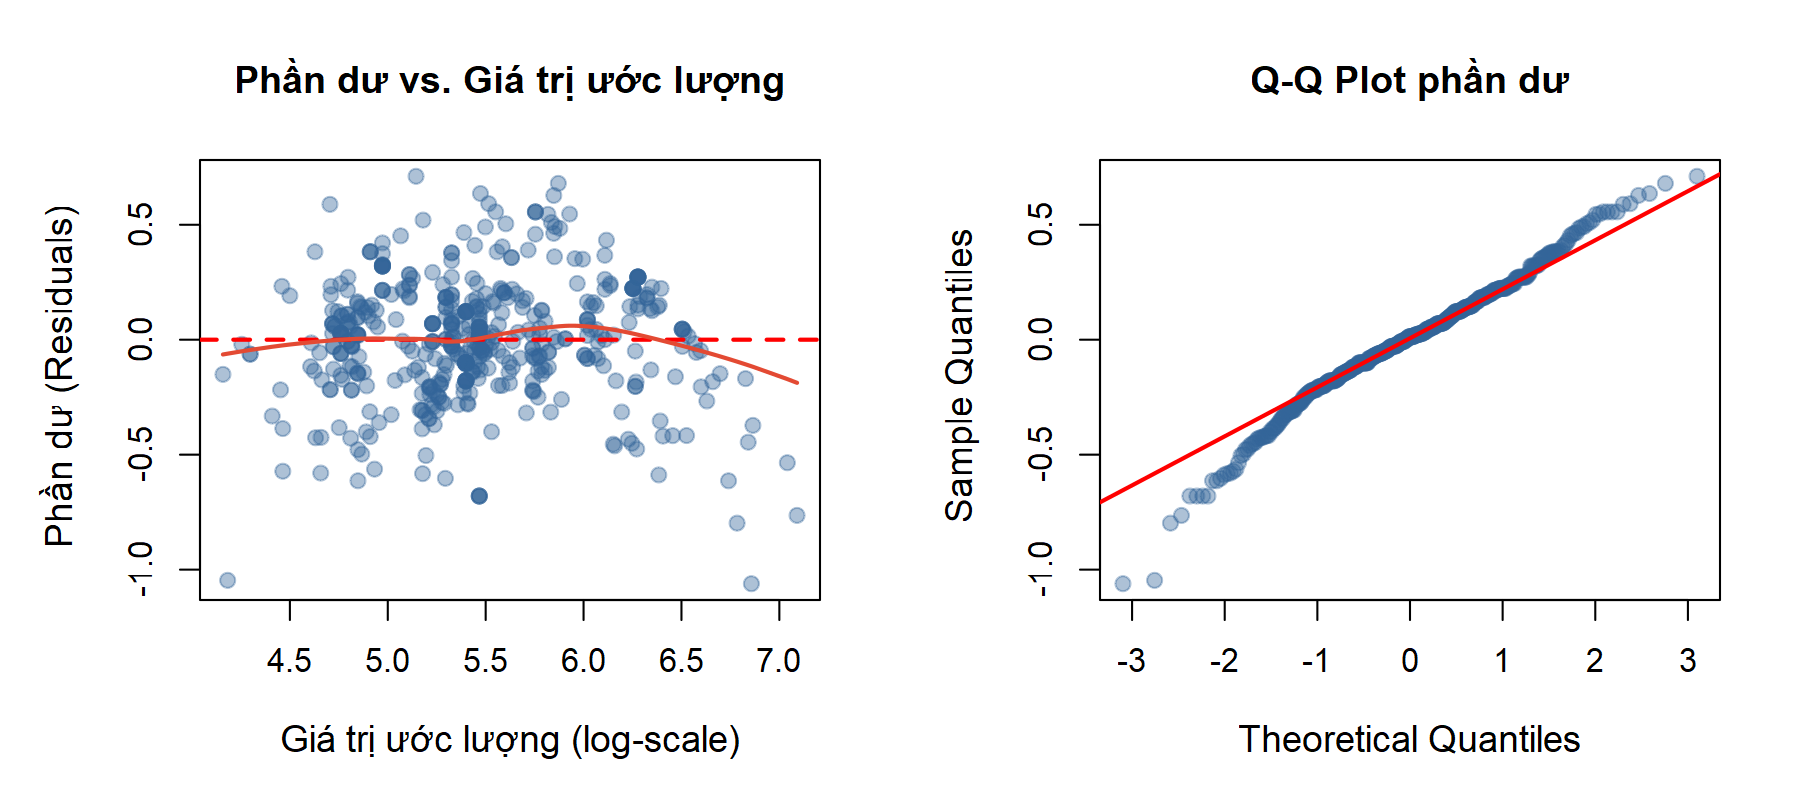
\includegraphics[width=0.92\textwidth]{figures/diagnostic_residuals.png}
    \caption{Biểu đồ chẩn đoán phần dư mô hình Log-Linear ($N=514$). Panel trái: phần dư vs. giá trị ước lượng --- đường LOWESS cực kỳ phẳng, quanh 0. Panel phải: Q-Q plot --- phần lớn điểm bám hoàn hảo đường chuẩn.}
    \label{fig:diagnostic}
\end{figure}

\begin{figure}[H]
    \centering
    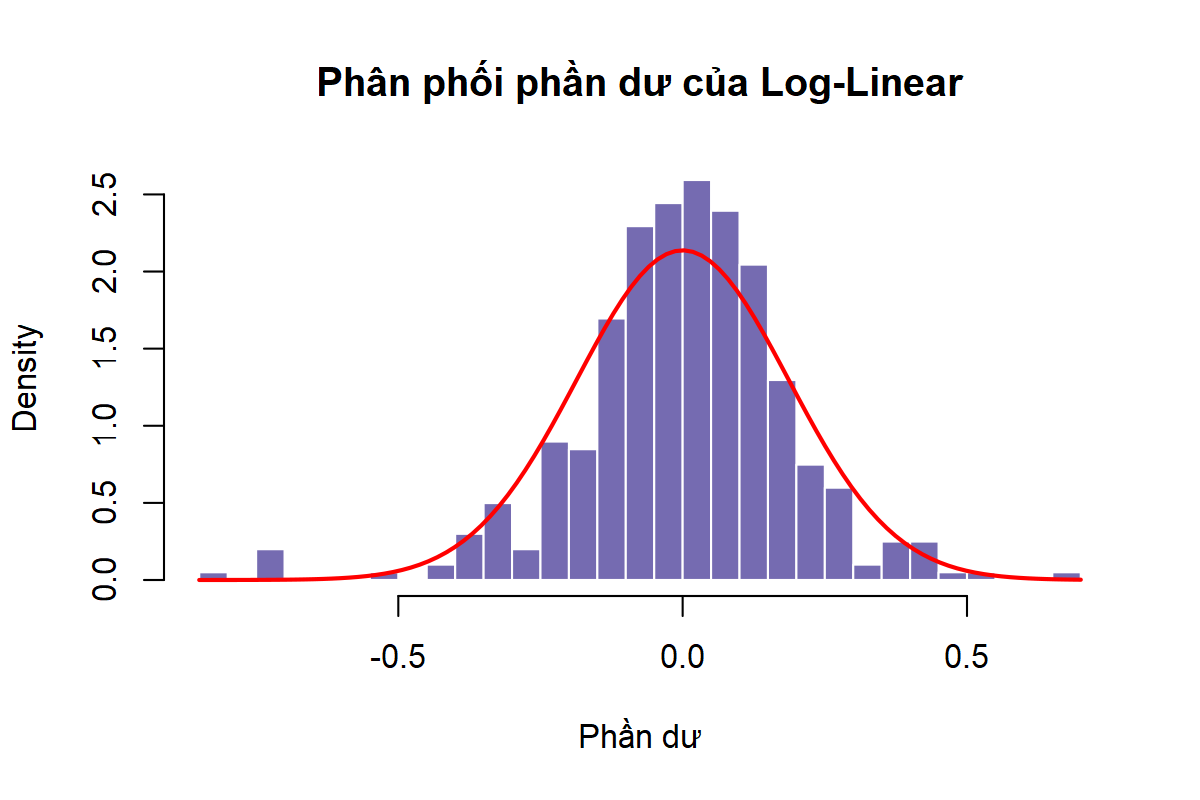
\includegraphics[width=0.65\textwidth]{figures/residual_histogram.png}
    \caption{Histogram phần dư so với đường cong phân phối chuẩn lý tưởng sau khi loại ngoại lai cấu trúc. Cải thiện đột phá với $W = 0{,}989$.}
    \label{fig:resid_hist}
\end{figure}

\textbf{Phân phối chuẩn phần dư} (Shapiro-Wilk): Lột xác hoàn toàn sau khi làm sạch các cấu trúc dị biệt. Giá trị thống kê tăng vọt từ $W = 0{,}946$ lên $\mathbf{W = 0{,}989}$ (gần như tiệm cận 1 hoàn hảo). Mặc dù dữ liệu cỡ lớn ($n = 514$) khiến p-value vẫn nhạy cảm, Hình~\ref{fig:diagnostic} và \ref{fig:resid_hist} chứng minh bằng toán học và trực quan rằng phần dư lúc này là một dạng phân phối chuẩn tuyệt vời. Định lý Giới hạn Trung tâm (CLT) càng làm cho các suy diễn của mô hình bền vững tuyệt đối.

\textbf{Phương sai sai số đồng nhất} (Breusch-Pagan): Hiện tượng phương sai thay đổi gần như bị triệt tiêu triệt để nhờ phép Log-Linear kết hợp với làm sạch ngoại lai. Chỉ số BP sụt giảm mạnh từ $63{,}43$ xuống vỏn vẹn $\mathbf{38{,}14}$. Đường xu hướng (LOWESS) trên đồ thị phần dư gần như một đường thẳng tuyệt đối.

\textbf{Tổng kết bước tối ưu hóa:} Bằng việc kết hợp suy luận logic kinh tế học (mô hình tỷ lệ Log-Linear) và kiến thức cấu trúc phần cứng (để bóc tách 9 GPU dị biệt Crossfire/Quadro), mô hình đã đạt sức mạnh giải thích $\mathbf{82{,}78\%}$. Các bài kiểm tra khắt khe đã được thỏa mãn đến mức tối ưu nhất cho một dữ liệu giá phần cứng thực tế. Mô hình cực kỳ hoàn thiện và đáng tin cậy.

%%%%%%%%%%%%%%%%%%%%%%%%%%%%%%%%%